
\chapter{Systemarkitektur}
\begin{longtabu} to \linewidth{@{}l l l X[l]@{}}
	
	
	Version &    Dato &    Ansvarlig &    Beskrivelse\\[-1ex]
	\midrule
	0.1 &    03-11-2015 &    MBA &    Oprettelse \\[-1ex]
	0.2 &    10-11-2015 &    DHC, MBA &     HW Start af skrivning, indsætning af billeder  \\[-1ex]
	0.3 &  10-11-2015   &  ABH   &   SW Start på design, indsætning af diagrammer  \\[-1ex]
	0.4 &  11-11-2015   &  DHC   &   HW Design Forstrækning  \\[-1ex]
	0.5 &  13-11-2015   &  ABH   &   SW Design klasse- og metodeidentifikation  \\[-1ex]
	0.6 & 18-11-2015 & ABH & HW Rettelse af diagrammer \\[-1ex]
	0.7 & 18-11-2015 & DHC, AJF & HW Implementering Forstrækning, Modultest Lavpas \\ [-1ex]
	0.8 & 18-11-2015 & MHNK, JMM & SW Design, Rettelse af domænemodel \\[-1ex]
	0.9 & 18-11-2015 & ABH & SW Design, Mere metodeidentifikation \\[-1ex]
    1.0 & 20-11-2015 & MHNK & SW Indskrivning af alle sekvensdiagrammer \\[-1ex]
	1.1 & 26-11-2015 & DHC & HW Modultest, Kalibrering ved vandsøjle \\ [-1ex]
	1.2 & 26-11-2015 & DHC, AJF & HW Design Lavpas \\ [-1ex]
	1.3 & 02-12-2015 & DHC & HW Referencer  \\ [-1ex]
	1.4 & 02-12-2015 & MHNK & HW Rettelser i tekst \\[-1ex]
	1.5 & 02-12-2015 & DHC, MBA & HW Modultest \\[-1ex]
	1.6 & 04-12-2015 & ABH & SW Implementering, Generelt, Analyse og Digitalt filter \\[-1ex]	 
	1.7 & 06-12-2015 & ABH & SW Implementering, Kalibrering og nulpunktsjustering \\[-1ex]
	1.8 & 09-12-2015 & DHC & Rettelser i tekst \\ [-1ex]
	1.9 & 09-12-2015 & ABH, JMM & SW Implementering Observer-Strategy, Analyse og Digital Filter \\ [-1ex]	
	
	\label{version_Systemark}
\end{longtabu}

I det følgende beskrives arkitekturen for systemet. Systemarkitekturen er vores udviklingsramme for den videreudvikling af design og implementering af blodtrykssystemet. Designet af systemet er grebet an således at, der først kigges på det overordnede system, hvorefter systemet arbejdes ned i mindre brudstykker. Dette gøres ved at benytte diagrammer med tilhørende beskrivelser.

\section{Hardware}
\subsection{Design}
Systemets hardware kan illustreres i et BBD. Det ses på figur \ref{fig:BDD} at systemet består af fem hardware blokke: software system, forstærker, filter, DAQ og transducer. Disse fem blokke udgør til sammen selve blodtryksmåleren.  
	
\begin{figure}[H]
	\centering
	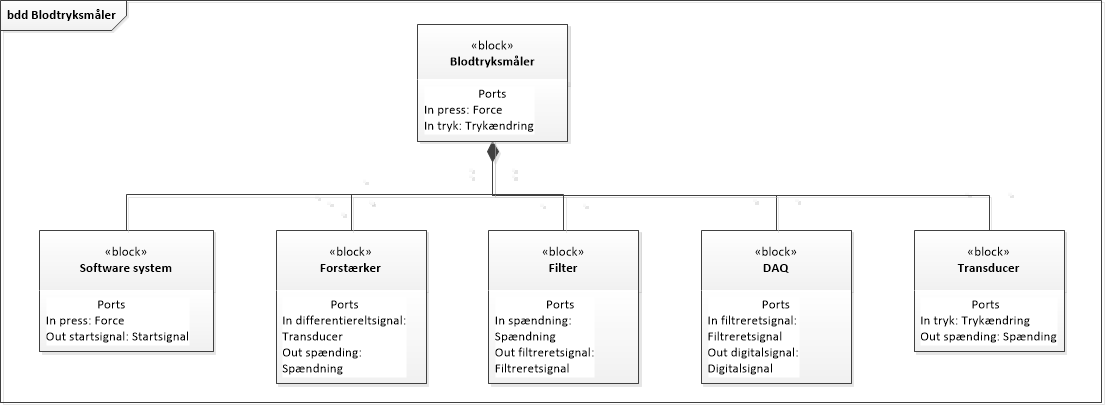
\includegraphics[width=1.0\textwidth]{Figurer/BDD}
	\caption{Block Definition Diagram for hardware}
	\label{fig:BDD}
\end{figure}

Ovenstående BDD-diagram fører videre til udarbejdelsen af IBD for hardware komponenterne. I IBD diagrammet vises koblingen mellem de forskellige blokke gennem port forbindelser. Det ses at signalet starter ved transduceren, hvorefter det bliver behandlet gennem forstærker, filter og DAQ. Til sidst sendes det ind i software systemet, som bliver påvirket af tryk på knapper på GUI. 

\begin{figure}[H]
	\centering
	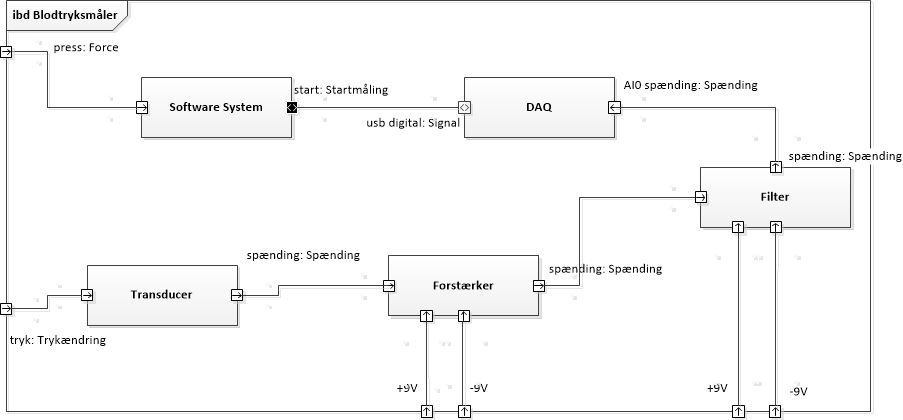
\includegraphics[width=1.0\textwidth]{Figurer/IBD}
	\caption{Internal Block Diagram for hardware}
	\label{fig:IBD}
\end{figure}

\subsubsection{Forstærkning}
Transduceren måler en trykændring som den omsætter til en spænding. Dette er udtrykt ved et differentieret signal, som sendes ind i forstærker-blokken. Da signalet fra transduceren er en lav spænding, skal det forstærkes op, for at passe med DAQ'ens input. Denne forstærkning udregnes ud fra det maksimale output fra transduceren og det maksimale input til DAQ'en. Se beregningerne under Implementering.  

Under simulering bruges Analog Discovery som en funktionsgenerator, der simulere det differentieret signal. Analog Discovery har en usikkerhed, når der arbejdes med små spændinger. Dette kan modarbejdes vha. spændingsdeler princippet. Dette gør at Analog Discovery kan sende en højere spænding ind i systemet, så usikkerheden mindskes. Dette bruges kun under simulering og teste af hardwaren.   

\subsubsection{Lavpas}
I projektet skal der laves et 2. ordens lavpasfilter. Filteret skal laves for at sikre, at der ikke opstår aliasering.\\
Aliasering \cite{DSB} er, hvor signalet bliver gentaget. Når man har signalet i det digitale domæne, bliver spektret for signalet en periodisk funktion. Det vil sige, at den gentager sig selv, efter et bestemt stykke tid. \\
Det skal sikres, at der ikke kommer overlap mellem signalet og et alias. Da det ellers kunne give anledning til misforståelser. Derfor laves et lavpasfilter, som sikre at der ikke ligger noget signal ved den halve samplingsfrekvens. Signalet her kan med fordel gøres så lille at DAQ'en ikke kan læse det, dvs. signalet skal være mindre end $ 1/2 \cdot LSB $ (Least Significant Bit).    

Lavpasfilteret skal være et Sallen-Key Butterworth-filter med en knækfrekvens på 50 Hz og en samplingsfrekvens på 1kHz. Ud fra oplysninger givet til projektet, vides det at filteret skal dæmpe signalet med 20 dB, under antagelse af at, den forekommende støj er mindre end signalet, også når støjen forekommer over knækfrekvensen.

Ved en typisk blodtryksmåling forekommer der ikke signal over 50 Hz, samtidigt er signalet her aftaget med ca. 70 dB. For at få signalet, ved den halve samplingsfrekvens til at være $ 1/2 \cdot LSB $, skal det ydeligere dæmpes 20 dB. Derfor oplyses filterets til at være 50 Hz, da dette giver en minimums dæmpning på 20 dB pr. dekade.

\subsection{Implementering}
\subsubsection{Forstærkning}
For at få den rette forstærkning er det blevet valgt, at benytte instrumentationsforstærkeren INA-114. Her kan transduceren sættes på med det differentierede signal. INA114 er valgt da følgende gælder\cite{Instrumentation} for instrumentationsforstærkere: 
\begin{itemize}
	\item Differentielt input - single ended output 
	\item Gain justering med ændring af kun én modstand 
	\item Meget høj indgangsimpedans 
	\item Stor Common Mode Rejection Ratio(CMRR)
\end{itemize}
Under opbygning og modultestning vil det differentierede signal blive simuleret af Analog Discovery. \\
For at udregne den korrekte forstærkning, bruges følsomheden fra transduceren og eksistationsspændingen.
Først udregnes det maksimale output fra transduceren: 
\begin{ceqn}  
\begin{equation}
9V\cdot 250mmHg \cdot 5\mu\cdot 10^{-5} uV/V/mmHg  = 11.25mV
\end{equation}
\end{ceqn}
Da det er besluttet at det maksimale input til DAQ'en \cite{DSB} er 5V, kan forstærkningen (Gain) nu udregnes:
\begin{ceqn}
\begin{equation}
\begin{split}
5V& =11.25mV\cdot G\\   
G& =444.44
\end{split}
\end{equation}
\end{ceqn}
\cite{INA} For at få den rette forstærkning udregnes den eksterne modstand ($ R_g $) til INA114.\\ 
INA114's forstærkning afhænger af størrelsen på $ R_g $, hvis modstanden er stor, er forstærkningen lille og omvendt.  $ R_g $ udregnes ved formlen:
\begin{ceqn}
\begin{equation}
\begin{split}
G&=1+\frac{50k\Omega}{R_g}\\
444.44&= 1+\frac{50k\Omega}{R_g} \Rightarrow R_g= 112.75 \Omega
\end{split}
\end{equation}
\end{ceqn}
Derved fås en værdi for den eksterne modstand til INA114, som skaber den ønskede forstærkning.\\
Det skal nu sikres at dette kan lade sig gøre. Derfor sikres det, at den ønskede forstærkning kan ske ved båndbredden. Dette kan undersøges da produktet af forstærkning og båndbredde er en konstant. Konstanten aflæses i databladet for INA114\cite{INA}. 
\begin{ceqn}
\begin{equation}
\begin{split}
1000000 Hz& = G\cdot BW \\
BW& = 2250 Hz
\end{split}
\end{equation}
\end{ceqn}
Da båndbredden ligger over knækfrekvensen for lavpas filtret, er dette godkendt. Hvis båndbredde havde ligget under knækfrekvensen vil operationsforstærkeren ikke have kunnet arbejde med de ønskede frekvenserne. Derfor er det vigtigt at båndbredden er bred nok til at kunne indeholde frekvenser fra begge side af knækfrekvensen.\\
\newline 
For at imødekomme usikkerheden ved Analog Discovery med lave spændinger, laves et kredsløb efter spændingsdelerprincippet. Signalerne fra Analog Discovery skal sendes igennem dette kredsløb, hvor de efter spændingsdelerprincippet gøres mindre. I kredsløbet benyttes to modstande, hvis værdier er $ R_1=100k\Omega $ og $ R_2 = 1k\Omega $. Da vi kender signalet som skal ind i INA114 og modstandene i kredsløbet, kan størrelsen af den spænding, som skal sendes fra Analog Discovery, findes:
\begin{ceqn}
\begin{equation}
\begin{split}
U_{INA}& = U_{analog} \cdot \frac{R_2}{R_1 + R_2} \\
11.25mV& = U_{analog}\cdot \frac{1k\Omega}{100k\Omega+1k\Omega} \Rightarrow U_{analog}=1.1362 V
\end{split}
\end{equation}
\end{ceqn}
Derved kan Analog Discovery sende signaler med en højere spænding ud og usikkerheden mindskes. Der er taget højde for at, hvis modstandene i kredsløbet bliver for store, vil det skabe en termisk usikkerhed. Derfor er modstandene valgt som de er. Dette er kun under simulering, når transduceren benyttes, bruges spændingsdeleren ikke.  
  
\subsubsection{Lavpas}
For at opnå den ønskede effekt i lavpasfilteret, blev det oplyst at $ f_c=50$ Hz, $ f_s = 1$kHz, $ R_1 = R_2 $ og $ C_2=680 nF$. Ud fra disse værdier, udregnes de resterende komponentværdier for filteret.

Overføringsfunktionen for et 2. ordens filter er:
\begin{ceqn}
\begin{equation}
H(z)=\frac{\omega_n^2}{(s^2 + 2\cdot\zeta \cdot \omega_n \cdot s+\omega_n^2)}
\end{equation}
\end{ceqn}

For at finde overføringsfunktionen for det gældende system, vides det at følge ligninger gælder \cite{Wikilavpas}:
\begin{ceqn} 
\begin{equation}
\begin{split}
\omega_n = 2\cdot \pi\ 50 &= \dfrac{1}{\sqrt{R1\cdot R2\cdot C1\cdot C2}}\\
2\cdot \zeta\cdot\omega_n& =\frac{1}{C2}\cdot \left( \frac{R1+R2}{R1\cdot R2}\right)
\end{split}
\end{equation}
\end{ceqn}
Derved fås en overføringsfunktion som hedder: 
\begin{ceqn}
\begin{equation}
H(z)=\frac{\left(\dfrac{1}{\sqrt{R1\cdot R2 \cdot C1\cdot C2}}\right)^2}{s^2+ \left( \dfrac{1}{C2} \cdot \left( \dfrac{R1+R2}{R1\cdot R2}\right) \cdot s \right) +\left( \dfrac{1}{\sqrt{R1\cdot R2 \cdot C1\cdot C2}}\right)^2 }
\end{equation}
\end{ceqn}
Da det bliver oplyst at $ R1=R2 $, kan funktionen reduceres. Den kan samtidig simplificeres. I sidste ende fås overføringsfunktionen, se Beregninger til overføringsfunktion under Bilag for nærmere udregninger:
\begin{ceqn}
\begin{equation}
H(z)=\dfrac{\dfrac{1}{C1 \cdot C2\cdot R^2}}{s^2+s\cdot \dfrac{2}{R\cdot C2}+ \dfrac{1}{C1\cdot C2\cdot R^2}}
\end{equation}
\end{ceqn}
Da der arbejdes med at 2. ordens Butterworth filter, vides det at udsvinget$ \zeta $ skal være 0.7 \cite{ASB}. 
Den sidste overføringsfunktion sammenlignes med den generelle for 2. ordens systemer. Det gælder at $ C2 = 680\cdot 10^{-9} nF $. Det er muligt at isolerer forskellige led. Først isoleres for modstanden:
\begin{ceqn}
\begin{equation}
\begin{split}
\dfrac{2}{R\cdot C2}=& 2\cdot \zeta \cdot \omega_n\\
\dfrac{2}{R\cdot 680\cdot 10^-9}=&2\cdot 0.7 \cdot(2\cdot\pi\cdot 50)\\
\Downarrow\\
 R=& 6687 \Omega
\end{split}
\end{equation}
\end{ceqn}
Derved er modstandene udregnet til $ R = 6687\Omega $. Nu kan der isoleres for kondensator C1:
\begin{ceqn} 
\begin{equation}
\begin{split}
\dfrac{1}{C1\cdot C2\cdot R^2}=& \omega^2\\
\dfrac{1}{C1\cdot 680\cdot 10^{-9}\cdot 6687^2}=& (2\cdot \pi \cdot 50)^2\\
\Downarrow\\
C1= &333\cdot 10^{-9} nF
\end{split}
\end{equation}
\end{ceqn}
Dette betyder, at $ C1 = 333\cdot 10^{-9} nF $  og  $ C2 = 680\cdot 10^{-9} nF$. Derved er alle komponentværdierne til lavpasfilteret fundet og det kan nu realiseres. \\ 
\newline
Under udviklingen af lavpasfilteret er komponent størrelserne, blevet ændret for at kunne realisere det. De brugte komponent størrelser er: $ R= 6.6 k\Omega $, $ C1= 330\cdot 10 ^{-9} nF$ og $ C2= 680\cdot 10^{-9} nF$.   
For at være sikker på at filteret har de ønskede karakteristika, laves et bodeplot for den endelig overføringsfunktion:
\begin{ceqn}
\begin{equation}
H(z)=\dfrac{62500000000}{610929\cdot \left( s^2+\dfrac{250000}{561}\cdot s + \dfrac{62500000000}{610929} \right)}
\end{equation}
\end{ceqn}
\begin{figure}[H]
	\centering
	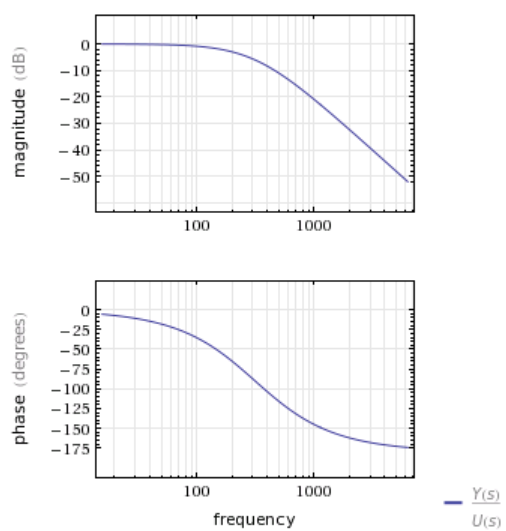
\includegraphics[width=0.5\textwidth]{Figurer/Bodeplot}
	\caption{Bodeplot}
	\label{fig:bodeplot}
\end{figure}
Udregning af den præcise oversving $ \zeta $ ud fra de benyttet komponentværdier:
\begin{ceqn} 
\begin{equation}
\begin{split}
\dfrac{2}{R\cdot C1}=& 2\cdot \zeta\cdot \omega_n\\
\dfrac{2}{6600\cdot 680\cdot 10^{-9}}=& 2\cdot \zeta\cdot (2\cdot \pi \cdot 50)\\
\Downarrow\\
\zeta =& 0.709
\end{split}
\end{equation}
\end{ceqn}
Dvs. de små ændringer i komponent værdierne ikke har haft betydende indflydelse på værdien for $ \zeta $. 

\begin{figure}[H]
	\centering
	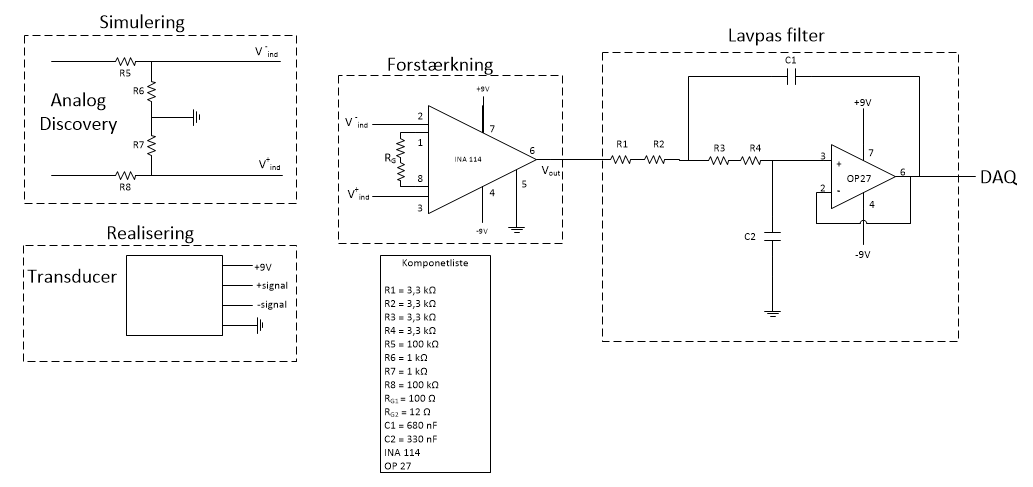
\includegraphics[width=1.0\textwidth]{Figurer/diagram_over_HW}
	\caption{Diagram over HW}
	\label{fig:HW}
\end{figure}

På figur \ref{fig:HW} ses et diagram over, hvordan kredsløbet er bygget op. Her ses kredsløbet for realiseringen med transduceren og for simuleringen med Analog Discovery.

\subsection{Modultest}
\subsubsection{Forstærkning}
For at teste forstærkningen sendes et differentieret signal ind vha. Analog Discovery. Signalet måles ved udgangen og der ses på, hvor meget signalet er blevet forstærket.\\ 
På figur \ref{fig:forstaerkning} ses det signal, som sendes ind i forstærknings blokken og det, der måles på udgangen af blokken. 
\begin{figure}[H]
	\centering
	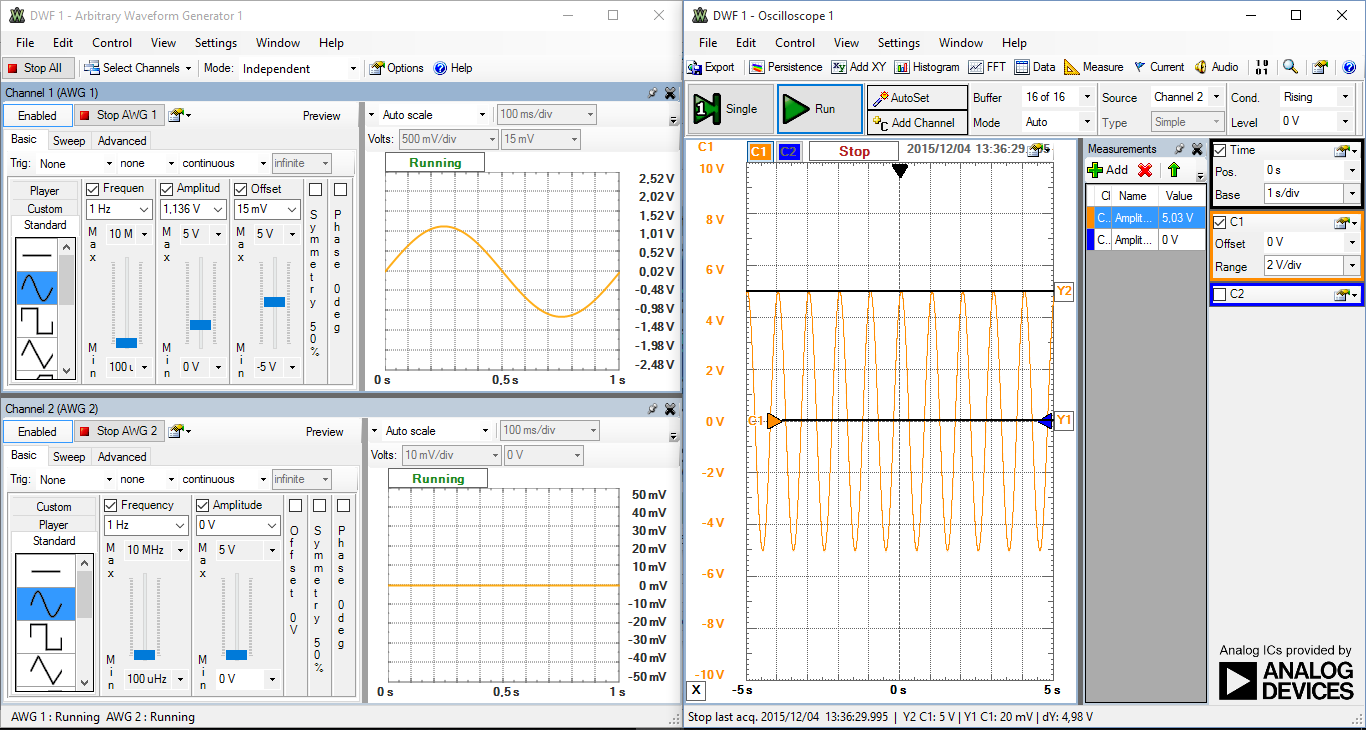
\includegraphics[width=1.0\textwidth]{Figurer/forst_blok}
	\caption{Forstærknings blok}
	\label{fig:forstaerkning}
\end{figure}
På udgangen, ses det at signalet er blevet forstærket op til 5 V DC. Herved er maks. output fra transduceren blevet forstærket så det passer med maks. input til DAQ'en. Signalet bliver ikke ændret på andre måde i forstærker blokken.

\subsubsection{Lavpas}
For at teste lavpasfilteret foretages målinger med en sinus, hvor frekvensen variere for hver måling. Fasen aflæses mellem indgang- og udgangssignal. Amplituden aflæses ligeledes for hver måling. 
Ved knækfrekvensen skal fasedrejningen være 90\textdegree. Dette kan aflæses på figur \ref{fig:maeling50Hz}.
Efter knækfrekvensen skal amplituden gå mod nul. Ved målingen for 60 Hz figur \ref{fig:maeling60Hz}, kan det ses hvordan amplituden er faldet drastisk efter knækfrekvensen. 
\begin{figure}[H]
	\centering
	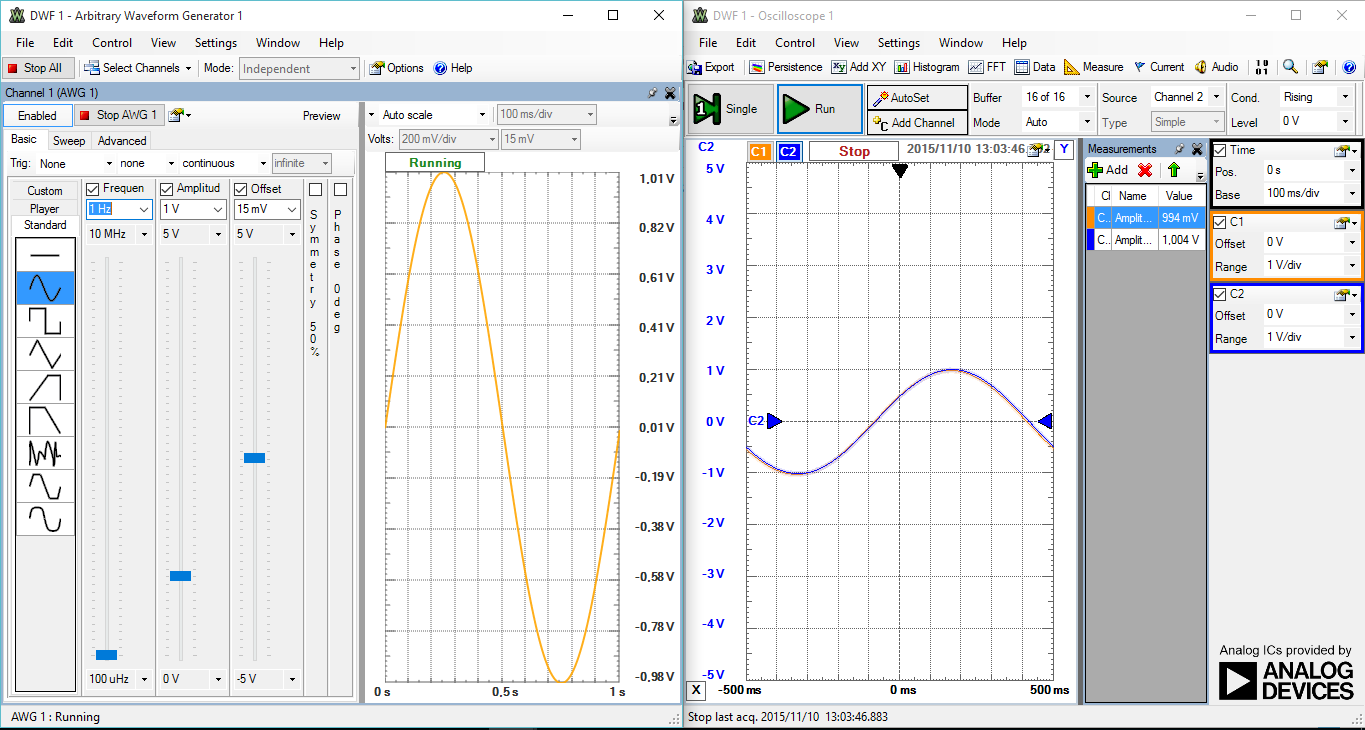
\includegraphics[width=1.0\textwidth]{Figurer/10Hz}
	\caption{Måling for 10 Hz}
	\label{fig:maeling10Hz}
\end{figure}

\begin{figure}[H]
	\centering
	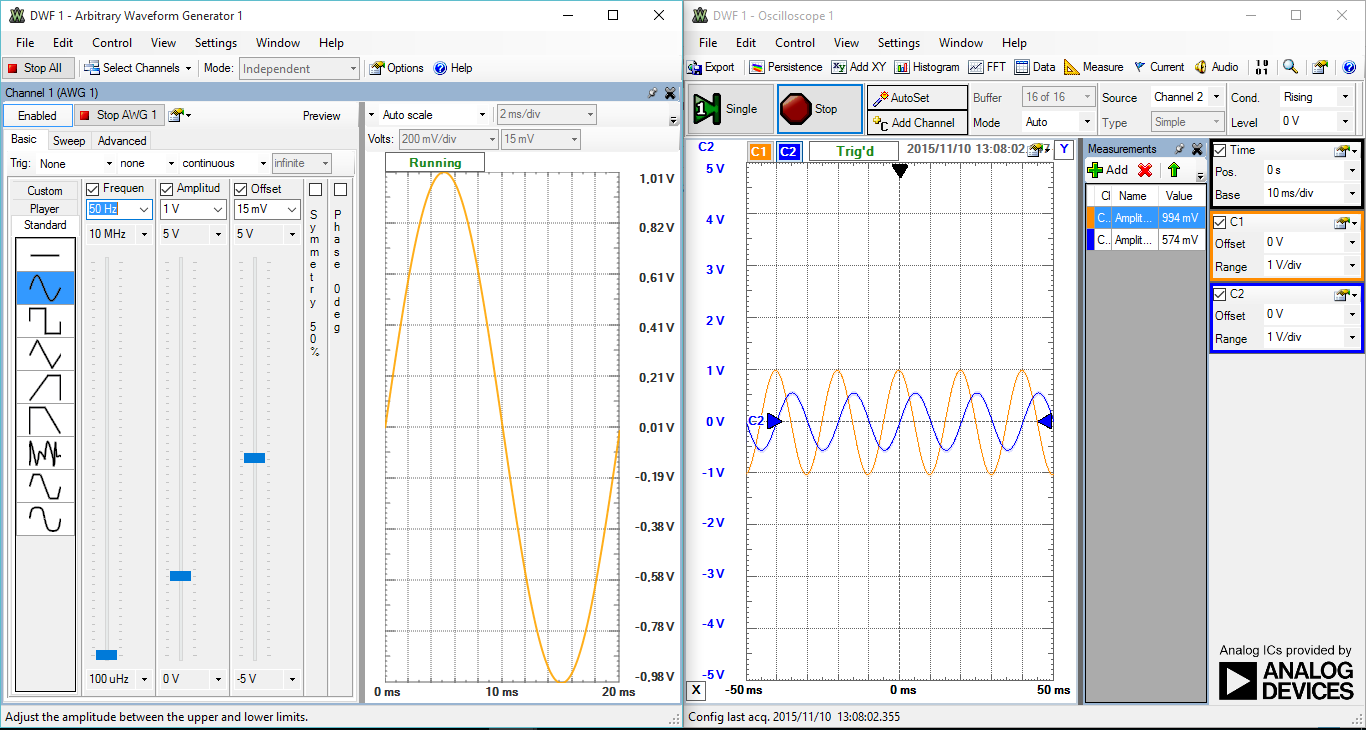
\includegraphics[width=1.0\textwidth]{Figurer/50Hz}
	\caption{Måling for 50 Hz}
	\label{fig:maeling50Hz}
\end{figure}

\begin{figure}[H]
	\centering
	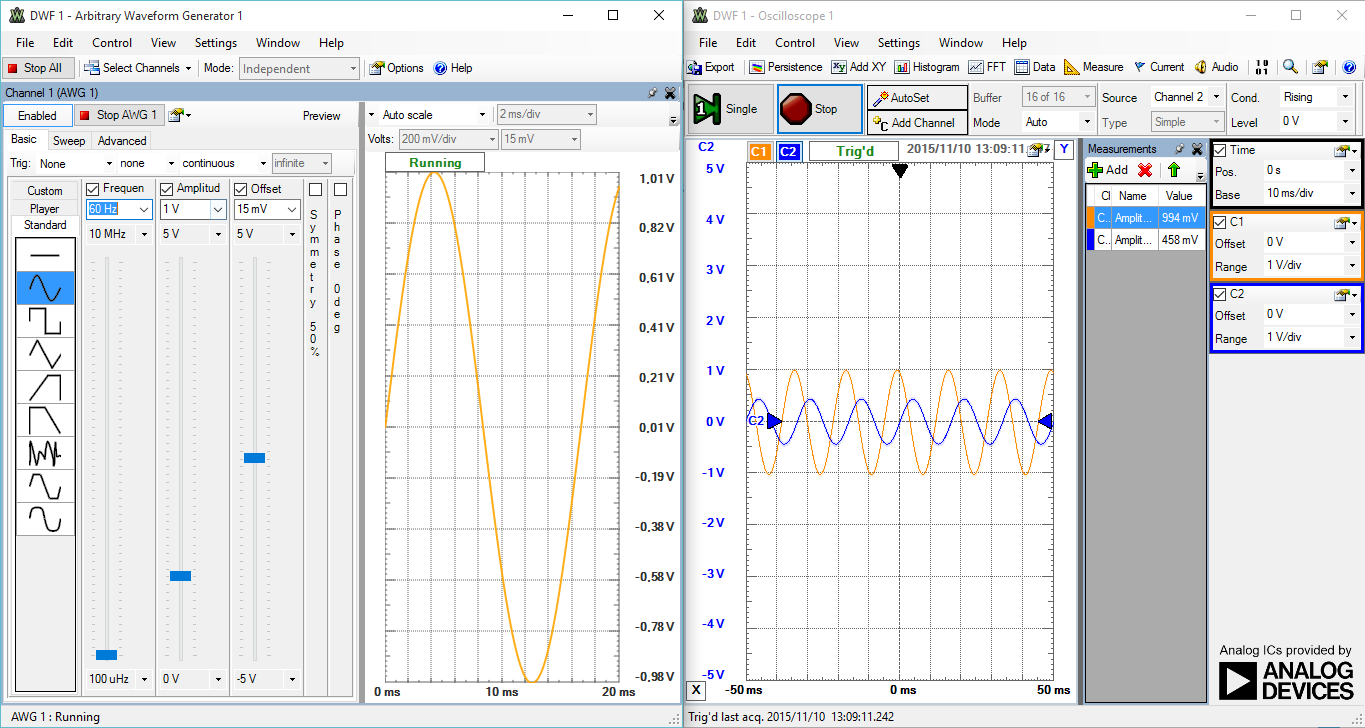
\includegraphics[width=1.0\textwidth]{Figurer/60Hz}
	\caption{Måling for 60 Hz}
	\label{fig:maeling60Hz}
\end{figure}

\subsubsection{Kalibrering med vandsøjle}
Efter forstærkning og lavpasfilteret er blevet testet hver for sig, udføres en kalibrering af systemet vha. en vandsøjle. Her bruges en udleveret vandsøjle med tre målepunkter, hvor det er angivet, hvor højt trykket(mmHg) er ved hvert af disse punkter. Derved kan det testes om hardware-delen måler den rigtige spænding i forhold til millimeter kviksølv(mmHg). Ud fra det maksimale antal volt (V) spænding og millimeter kviksølv(mmHg) kan det udregnes, hvad hardware skal vise ved 100 mmHg. 
\begin{figure}[H]
	\centering
	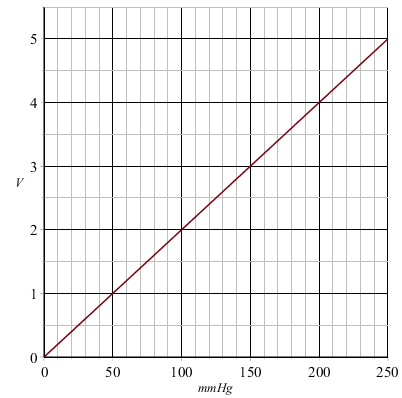
\includegraphics[width=0.3\textwidth]{Figurer/graf_vandtest}
	\caption{Graf til kalibrering, fra udregninger}
	\label{fig:graf_vandtest}
\end{figure}

Testen udføres ved, at fylde vand i søjlen til et bestemt punkt. Transduceren skal være tilkoblet et af de tre målepunkter, mens de andre er lukket til. Transduceren er sat til forstærkningen, der hvor Analog Discovery tidligere har været sat til. Transduceren er tilkoblet 0-9V, ved batterierne. På samme måde som ved simuleringen aflæses målingen på computeren ved hjælp af programmet WaveForms. Da det vides, hvilken trykændring der måles på, ved vi fra grafen til kalibreringen, hvilken spænding den skal vise. Dette fortages for de tre målepunkter på vandsøjlen, hvor hver måling sammenlignes med den udregnede graf. For hver måling, skal transduceren flyttes til et af de andre målepunkter.  

\begin{figure}[H]
	\centering
	\includegraphics[width=0.4\textwidth]{Figurer/vandtest_opstilling}
	\caption{Opstilling}
	\label{fig:vandtest_opstilling}
\end{figure} 
Opstillingen er gjort klar og der hentes ekstra vand under testen. Vandet skal bruges til at fylde vandsøjlen på til de forskellige målinger. \\
Ud fra grafen i figur \ref{fig:graf_vandtest} vides, hvad svaret på hver måling skal være. På figur \ref{fig:vandtest_måling50} ses målingen, da transduceren var tilkoblet målepunktet for 50 mmHg. Ud fra figur \ref{fig:graf_vandtest} vides det at målingen skal vise 1V DC.  
\begin{figure}[H]
	\centering	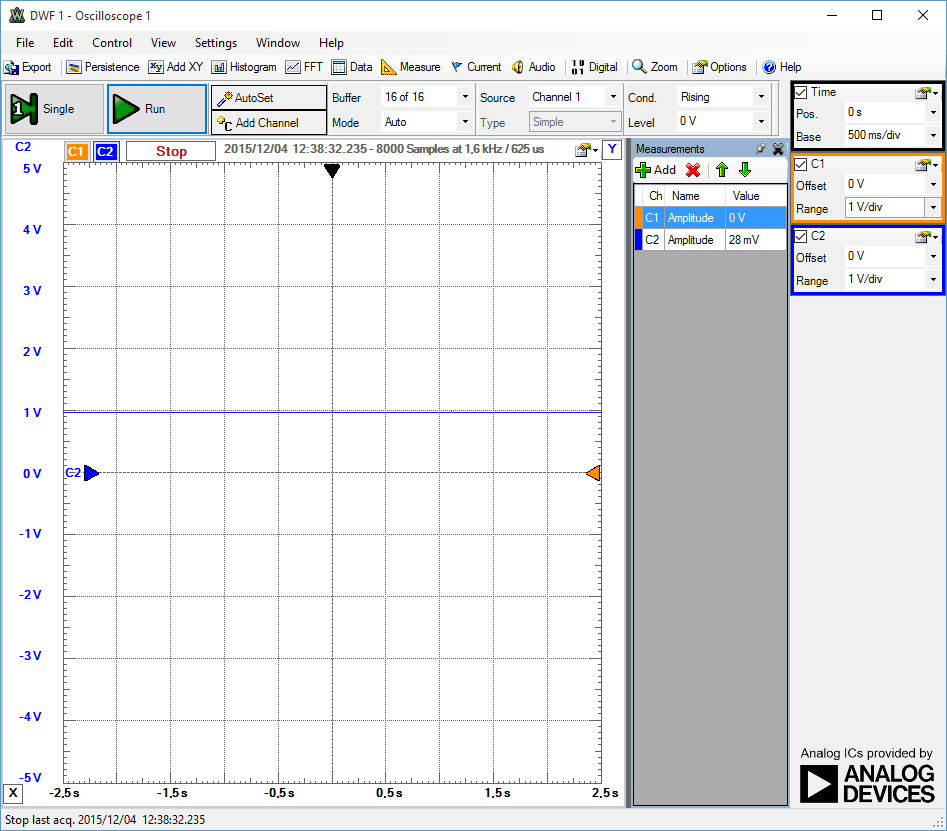
\includegraphics[width=0.8\textwidth]{Figurer/50mmhg}
	\caption{Måling ved 50 mmHg}
	\label{fig:vandtest_måling50}
\end{figure}
 
\begin{figure}[H]
	\centering	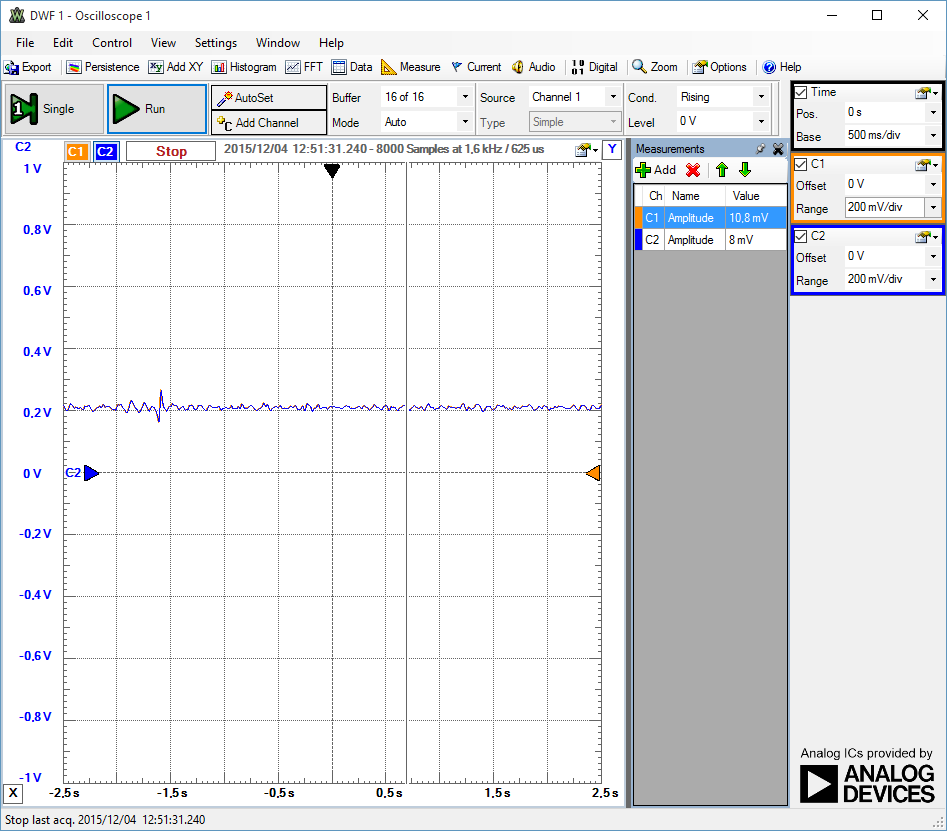
\includegraphics[width=0.8\textwidth]{Figurer/10mmhg}
	\caption{Måling ved 10mmHg}
	\label{fig:vandtest_måling10}
\end{figure}
På målingen for 10 mmHg ses en del rystelser(udsving på signalet). Som det ses på figur \ref{fig:vandtest_måling10} ligger signalet ikke præcist på 0.2V, dette kan skyldes at under testen, skal transduceren være i højde med målepunktet. Pga. korte ledninger, blev det under testen derfor nødvendigt at løfte og holde transducer, VEVO Board og Analog Discovery i højde med målepunktet. 

\begin{figure}[H]
	\centering	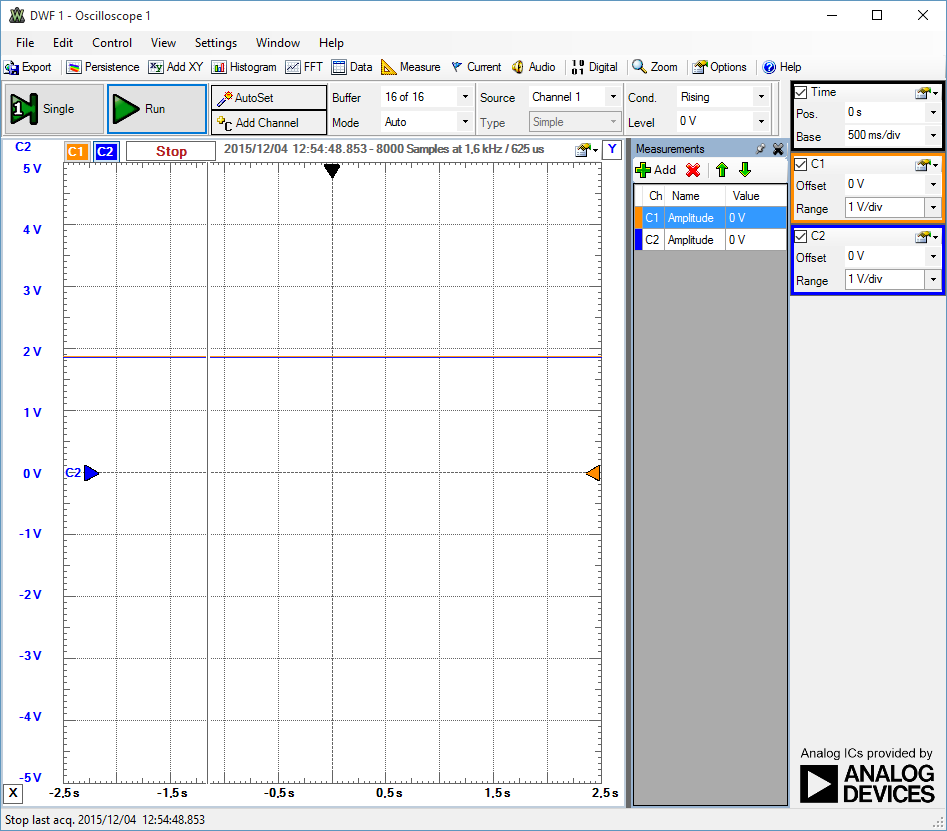
\includegraphics[width=0.8\textwidth]{Figurer/100mmhg}
	\caption{Måling ved 100mmHg}
	\label{fig:vandtest_måling100}
\end{figure}
Ved målingen for 100mmHg skulle der måles en spænding på 2V. Som det ses på figur \ref{fig:vandtest_måling100} ligger den ikke præcist på 2V. Som under målingen for 10 mmHg skal transduceren være i samme højde som målepunktet. Her er målepunktet lavt, men det skaber stadig en del usikkerhed.

   
\section{Software}
\subsection{Design}
I dette beskrives systemets softwaredesign på baggrund af systembeskrivelsen og kravspecifikationen. De overvejelser som er gjort i forbindelse med design af software vil blive præsenteret i dette afsnit.

\subsubsection{Overordnet sekvensdiagram}
Overordnet set ønskes det at udvikle et system, der kan interagerer med en forsker. Diagrammet herunder viser at forskerens opgave består i at starte, tage stilling til nulpunktsjustering og kalibrering samt gemme de ønskede data. Diagrammet er en simpel illustration som viser systemets adfærd gennem alle fem Use Cases. Formålet med dette diagram er udelukkende at skabe et overblik over det samlede system.

\begin{figure}[H]
	\centering
	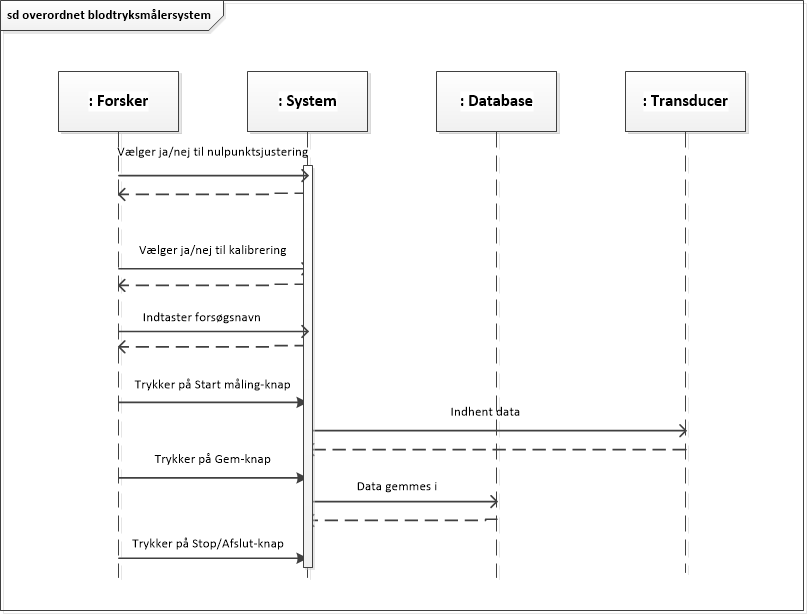
\includegraphics[width=0.7\textwidth]{Figurer/OverordnetSD}
	\caption{Overordnet sekvensdiagram for systemet}
	%\label{fig:Overordnet sekvensdiagram for systemet}
\end{figure}

\subsubsection{Problemidentifikation}
Første step i software designet er at klarlægge hvilke klasser systemet skal bestå af. Til dette er en domænemodel derfor udarbejdet med udgangspunkt i de fem Use Cases. I de fem Use Cases er de konceptuelle klasser blevet identificeret, og derefter indført som klasser i nedestående domænemodel. Modellen har til formål at vise hvilke dele systemet skal holde styr på. 

\begin{figure}[H]
	\centering
	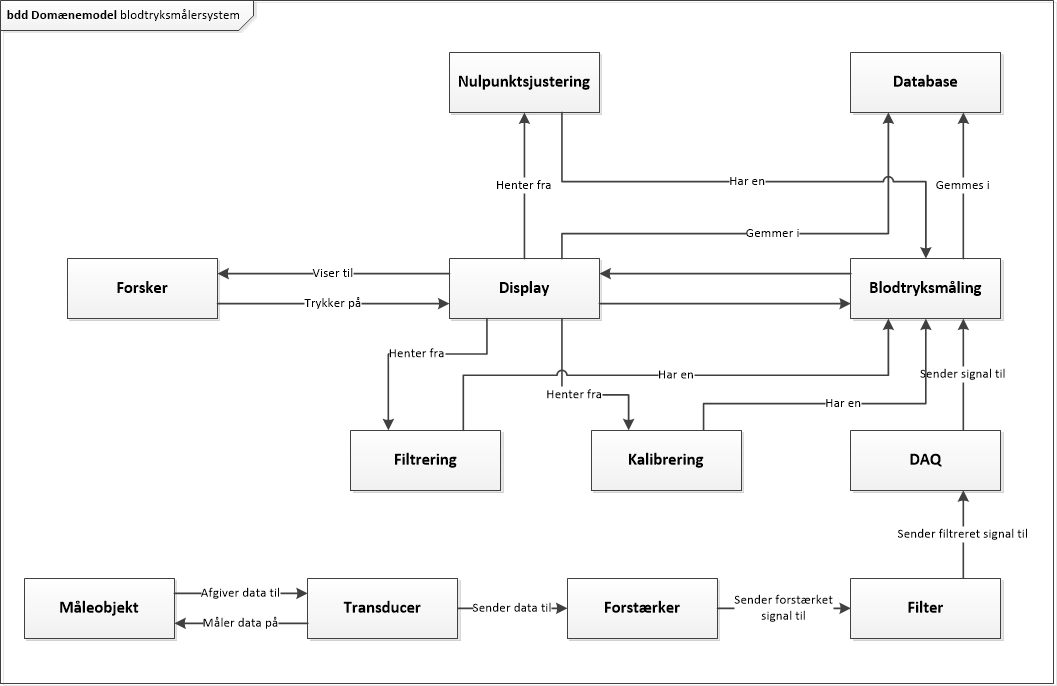
\includegraphics[width=1.0\textwidth]{Figurer/DomaneModel}
	\caption{Domænemodel}
	%\label{fig:Domænemodel}
\end{figure}

Diagrammet viser tydeligt forskerens interaktion med display, samt hvilke handlinger denne interaktion starter i system. Hardware-komponenterne er medtaget for at vise signalets vej fra måleobjekt til system. 

\subsubsection{Klasseidentifikation}
Ud fra domænemodellen kan et klassediagram udarbejdes, således tager dette diagram også udgangspunkt i de fem Use Cases. Hensigten med et klassediagram er at klarlægge hver klasses individuelle formål. 

\begin{figure}[H]
	\centering
	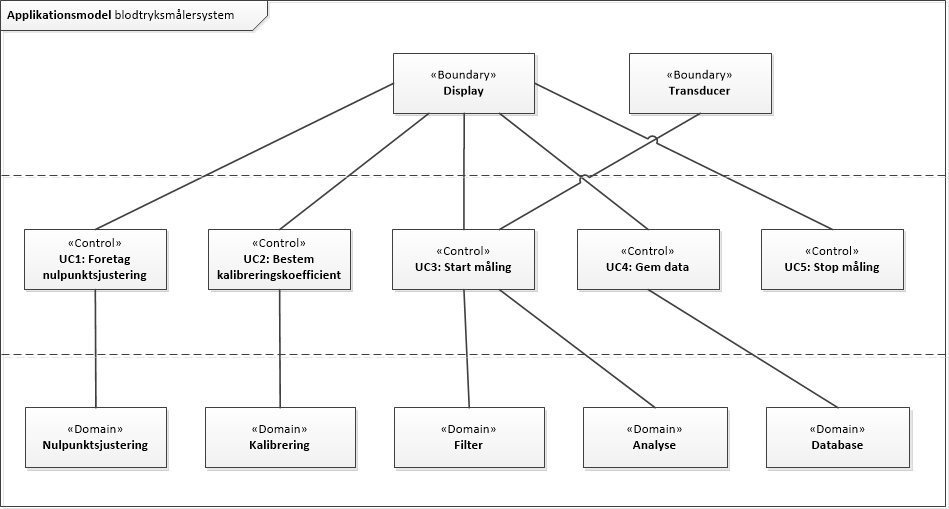
\includegraphics[width=1.0\textwidth]{Figurer/Applikationsmodel}
	\caption{Applikationsmodel for software}
	%\label{fig:Applikationsmodellen viser software klasser}
\end{figure}

Dermed ses det at denne model er delt op i tre niveauer:
\begin{enumerate}
\item Grænsefladeklasse
\begin{enumerate}
\item Transducer - Indhentet data fra måleobjekt
\item Display - Brugergrænseflade til forsker
\end{enumerate}
\item Kontrolklasse
\begin{enumerate}
\item UC1: Foretag nulpunktsjustering
\item UC2: Bestem kalibreringskoefficient
\item UC3: Start måling
\item UC4: Gem data
\item UC5: Stop måling
\end{enumerate}
\item Domæneklasse
\begin{enumerate}
\item Database
\item Nulpunktsjustering - Bestemmer nulpunktsjusteringsværdi
\item Kalibrering - Bestemmer kalibreringskoefficient
\item Filter - Indeholder det digitale filter
\item Analyse - Bestemmer systole, diastole og puls
\end{enumerate}
\end{enumerate}

\subsubsection{Metodeidentifikation}
Klasserne i ovenstående klassediagram er med til at definere, hvilke blokke de følgende sekvensdiagrammer må indeholde. Det er yderst vigtigt at der er en sammenhæng mellem klasserne i klassediagrammet og blokkene i sekvensdiagrammet. Vi har valgt at udarbejde et sekvensdiagram for hver enkelt Use Case, hvori systemets interne kommunikation beskrives, når normalforløb og udvidelser gennemløbes. I alle diagrammerne beskrives forløbet via de metodekald, der er nødvendige for at få de ønskede handlinger mellem blokkene udført. 

\textbf{Use Case 1}
\begin{figure}[H]
	\centering
	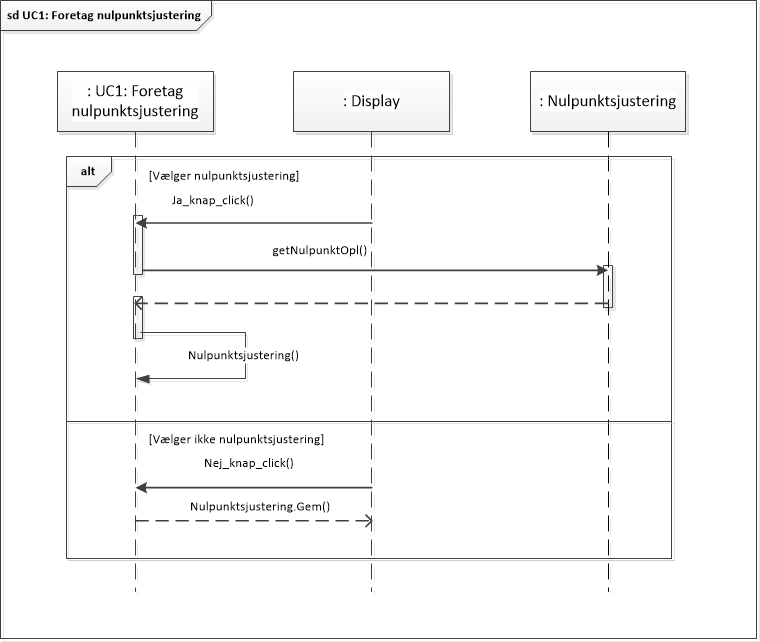
\includegraphics[width=1.0\textwidth]{Figurer/UC1}
	\caption{Sekvensdiagram for Use Case 1}
	%\label{fig:Sekvensdiagram for Use Case 1 - Foretag nulpunktsjustering}
\end{figure}
Det ses af ovenstående sekvensdiagram at forsker interagerer med display ved tryk på en knap. Denne interaktion skal igangsætte en nulpunktsjustering, som systemet udfører ved at læse den første indhentede værdi fra transduceren. 

\textbf{Use Case 2}
\begin{figure}[H]
	\centering
	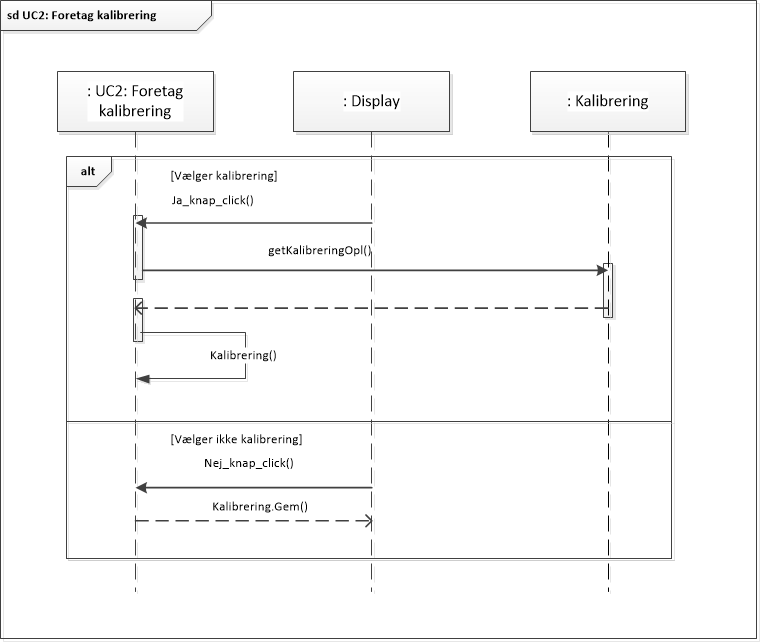
\includegraphics[width=0.7\textwidth]{Figurer/UC2}
	\caption{Sekvensdiagram for Use Case 2}
	%\label{fig:Sekvensdiagram for Use Case 2 - Foretag kalibrering}
\end{figure}
Af diagrammet på figur 3.18 ses det at kalibreringen skal implementeres simpelt i softwaren, hvor kaliberingskoefficienten hentes frem så den kan ganges på samtlige indhentede samples.

\textbf{Use Case 3}
\begin{figure}[H]
	\centering
	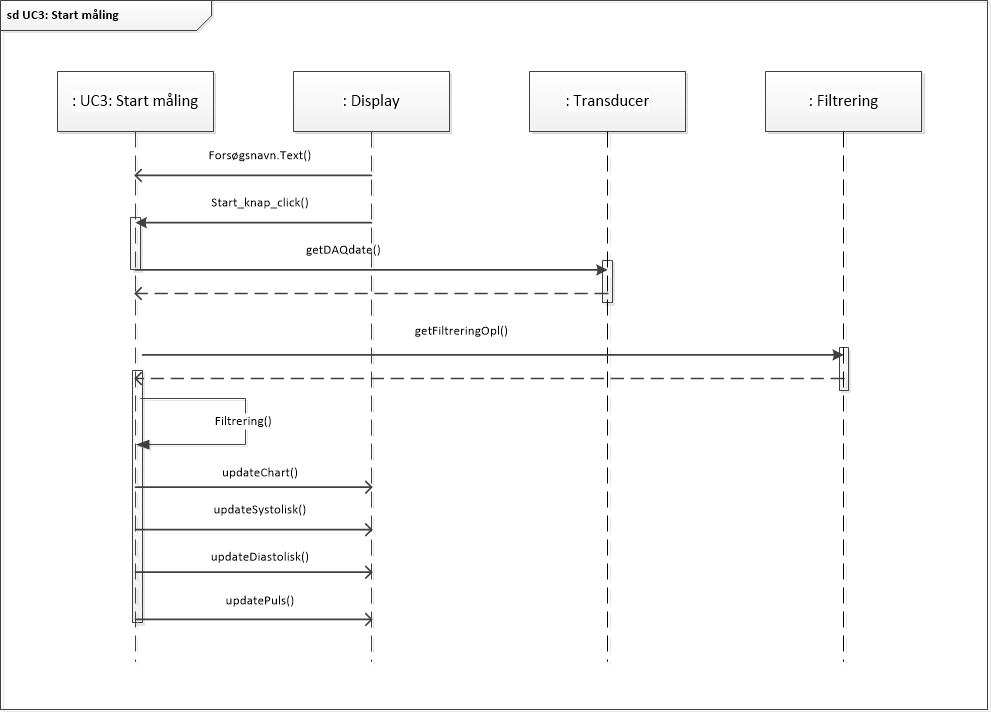
\includegraphics[width=1.0\textwidth]{Figurer/UC3}
	\caption{Sekvensdiagram for Use Case 3}
	%\label{fig:Sekvensdiagram for Use Case 3 - Start måling}
\end{figure}
Ved Use Case 3 - Start måling ses det at display-, transducer-, analyse- og filterklassen vil komme i spil. Her modtages besked ved indtastning af forsøgsnavn og tryk på start-knap på display om, at signaldata fra transduceren skal hentes ind i systemet. Herefter foretages filtrering af signalet, samt visning af signal i graf, systoliske-, diastoliske og puls-værdier på display. Use Casen indeholder en udvidelse hvor filtrering af signal ikke ønskes foretaget, dette er vist ved en optional nederst i diagrammet. 

\textbf{Use Case 4}
\begin{figure}[H]
	\centering
	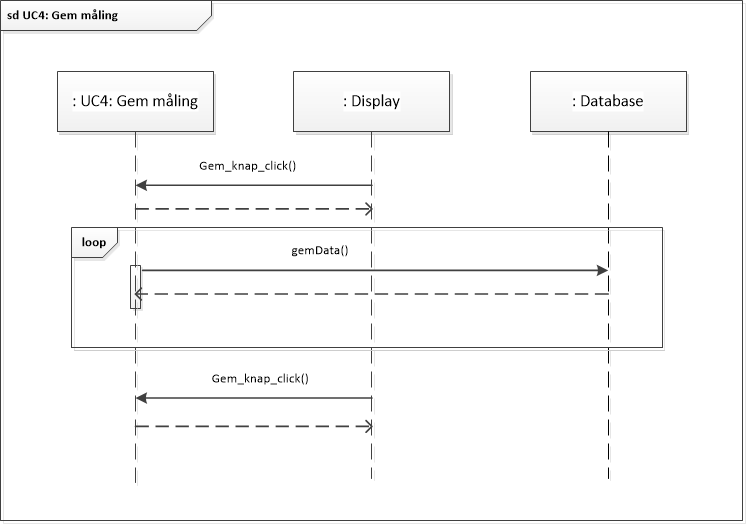
\includegraphics[width=0.7\textwidth]{Figurer/UC4}
	\caption{Sekvensdiagram for Use Case 4}
	%\label{fig:Sekvensdiagram for Use Case 4 - Gem data}
\end{figure}
Ovenstående diagram viser at for at få gemt data fra signalet, kræver det at der trykkes på START GEM-knap på display, hvorefter systemet skal gemme det fremadrettede signal indtil der trykkes på STOP GEM.

\textbf{Use Case 5}
\begin{figure}[H]
	\centering
	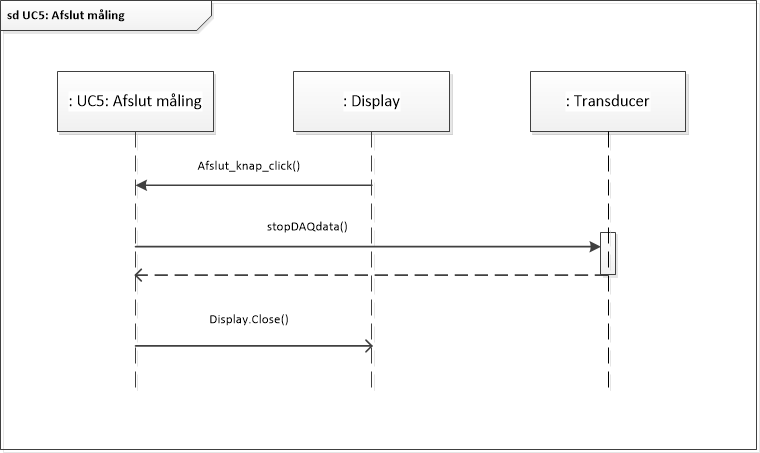
\includegraphics[width=0.7\textwidth]{Figurer/UC5}
	\caption{Sekvensdiagram for Use Case 5}
	%\label{fig:Sekvensdiagram for Use Case 5 - Afslut måking}
\end{figure}
Ved stop af en måling ses det at forsker trykker på STOP MÅLING-knap på display, hvorefter indhentening af data fra transduceren stoppes.

\subsection{Implementering}
\subsubsection{Indledende implementeringsovervejelser}
På baggrund af designfasen for softwaren kan implementeringen af softwaren påbegyndes. Softwaredesignet viser at systemet skal implementeres med en GUI applikation, som aktøren kan interagere med systemet gennem. Derudover er det kendt at softwaren skal indeholde en række klasser, hvor i funktionalitetér som kalibrering, nulpunktsjustering, digitalt filter og indhentning af systolisk-, diastoliske- og puls-værdier skal placeres. I det følgende beskrives de overvejelser vi har gjort i forhold til implementering af disse funktionaliteter og hele softwaresystemet generelt. 

Implementeringen af softwaren sker i Visual Studio 2013 i sproget C\#. Dette er valgt da programmet er godt til arbejde med GUI applikationer, samt til håndtering af tråde og tråd kommunikation. Tråde benyttes i softwaren, da systemet der skal implementeres er et eventdrevet system, hvilket vil sige at systemet skal kunne håndtere mange handlinger på en gang. Handlingerne igangsættes af events der kommer af aktørens interaktion med systemet. Tråd kommunikationen fungerer således at en tråd kan sende et signal ud som andre tråde kan reagere på. \\
Det er valgt kun at udarbejde aktivitetsdiagrammer for metoder, hvor vi mener det er med til at skabe et bedre overblik. Flere at metoderne er simple og derfor er et aktivitetsdiagram ikke nødvendig. 

\subsubsection{Klasse implementering}
På baggrund af designmodellerne er det besluttet at opbygge systemkoden efter principperne i en trelagsmodel. Trelagsmodellen indeholder et præsentations-lag, et logik-lag og et data-lag. Præsentations-laget består af de klasser som systemets aktører har tilgang til. Logik-laget er det analyserende lag. Det er således i dette lag at signalet behandles. Logik-laget har tilgang til de andre lag som det eneste. Det betyder at præsentations-laget og data-laget ikke kan kommunikere sammen, derved skal denne kommunikation foregå gennem logik-laget. Data-laget er tilgangen til den implementerede database og til indhentning af blodtrykssignalet fra hardware.

Fordelen ved trelagsmodel opbygningen er at det skaber et godt overblik i koden, og skaber en kode med lav kobling, da hver enkelt klasse har hvert sit specifikke ansvar. Hvilket gør at koden er let at vedligeholde og ændre hvis funktionaliteter ønskes opbygget anderledes. Et overordnet klassediagram over systemet er udarbejdet på baggrund af præcisering af applikationsmodellen, se figur 3.22. Hvilke metoder hver enkelt klasse indeholder kan ses på bilag xx.
\begin{figure}[H]
	\centering
	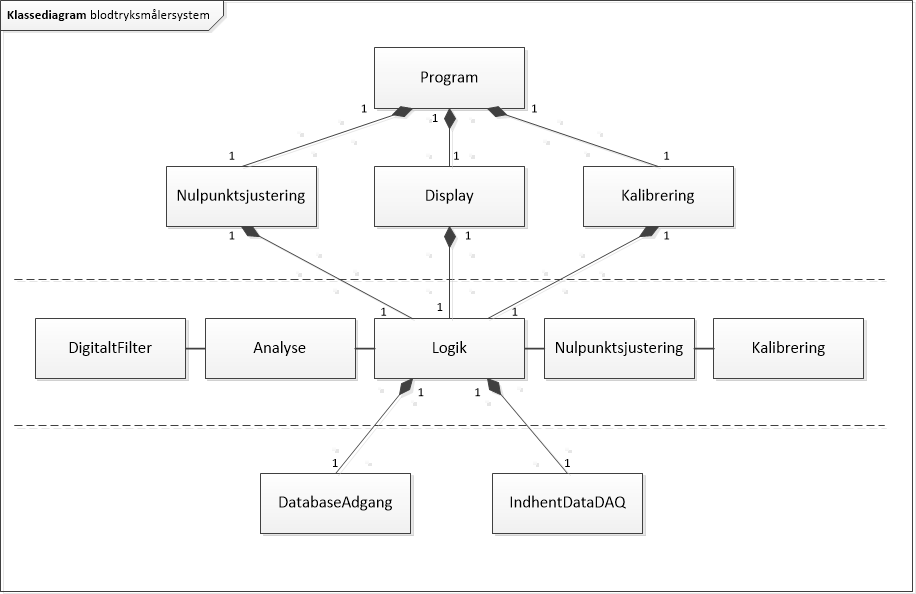
\includegraphics[width=1.0\textwidth]{Figurer/Klassediagram}
	\caption{Klassediagram}
	%\label{fig:Klassediagram over implementerede klasser i SW}
\end{figure}

\subsubsection{Brugergrænseflade}
Displayet (GUI) er aktørens, i dette tilfælde forskerens, indgang til systemet. Derfor er det vigtigt at den er opbygget efter hvad der følger forskerens logik. Til at klarlægge dette er principperne om en god brugergrænseflade taget i mente. Brugen af disse kommer til udtryk ved, at det tydeligt fremgår af hver knap eller label hvad dens formål er, samt at størrelsen af det enkelte komponent er tilstrækkelig stor til at det ikke er til at overse. Komponenterne på display er logisk placeret, det vil sige at de dele som forsker først skal forholde sig til og eventuelt udfylde er placeret i venstre side af display. Dette vil give mening såfremt systemet benyttes af personer fra den vestlige verden, hvor læseretningen er fra venstre mod højre. 

Det er et krav at forsker indtaster et forsøgsnavn inden at en måling startes, derfor er komponenterne implementeres således at knappen ”Start måling” først bliver aktiveret når der er indtastet noget i tekstboksen hvori forsøgsnavn skal indtastes. Systoliske-, diastoliske og puls-værdi er placeret efter hvilken rækkefølge det typisk ses på standard blodtryksapparater. 
\begin{figure}[H]
	\centering
	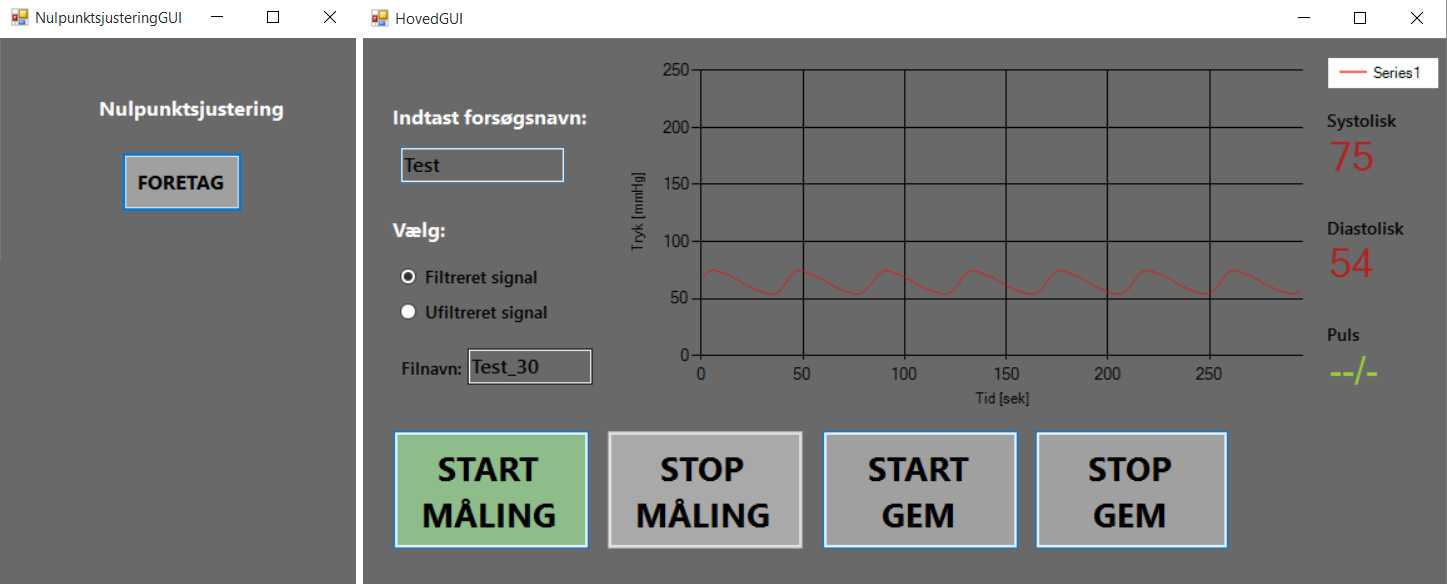
\includegraphics[width=1.0\textwidth]{Figurer/NulHovedGUI}
	\caption{NulpunktsjusteringGUI og HovedGUI}
	%\label{fig:Billede af systemets to forms}
\end{figure}
Af figur 3.23 ses det at grafen er en væsentlig del af display’s brugergrænseflade. Grafen implementeres som en Windows Form komponent. Det vælges at få vist signalet som en kurve, og førsteaksen indstilles til tid i sekunder fra 0 til 7 sekunder, og andenaksen til en minimums værdi på 0 mmHg og en maksimum værdi på 250 mmHg, hvilket er givet i kravspecifikationen. 

\subsubsection{Observer - Strategy}
Observer og strategy er to programmeringsmønstre. Der i samarbejde med hinanden er gode til at håndtere at sende data fa et lag til et andet lag. Det er valgt at bygge softwarekoden op efter disse to mønstre. Observer definerer et en til mange forhold mellem objekter således at en ændring i et objekts tilstand medfører at de mange objekter informeres om ændringer og dermed opdateres automatisk.

Dette implementeres ved at oprette to interfaces IObserver og ISubject. Disse interfaces placeres i deres eget namespace, som alle lag kan tilgå, samt gør det muligt for alle nødvendige klasser arve fra disse interfaces. I ISubject placeres de generelle metoder Notify() og Attach(), hvis ansvar er at informere og flytte data fra en klasse til en anden klasse når de kaldes i Subject-klassen. IObserver indeholder metoden der kaldes i Observer når en Notify() fra Subject og ISubject modtages. \\
Mønstret opbygges som en push, hvilket vil sige at når Subject har ny data klar til at sende op til Observer, kaldes metoden Notify() indeholdende data’en som parametre og dette sendes op til Observer, via ISubject og IObserver. Således fortsætter koden med at arbejde så længe ny data ønskes flyttes op. Mønstret benyttes både mellem data-laget og logik-laget, og mellem logik-laget og præsentations-laget. Skematisk er det i dette projekt givet ved, hvor de relevante metoder i forhold til mønstret er medtaget, se figur 3.23.
\begin{figure}[H]
	\centering
	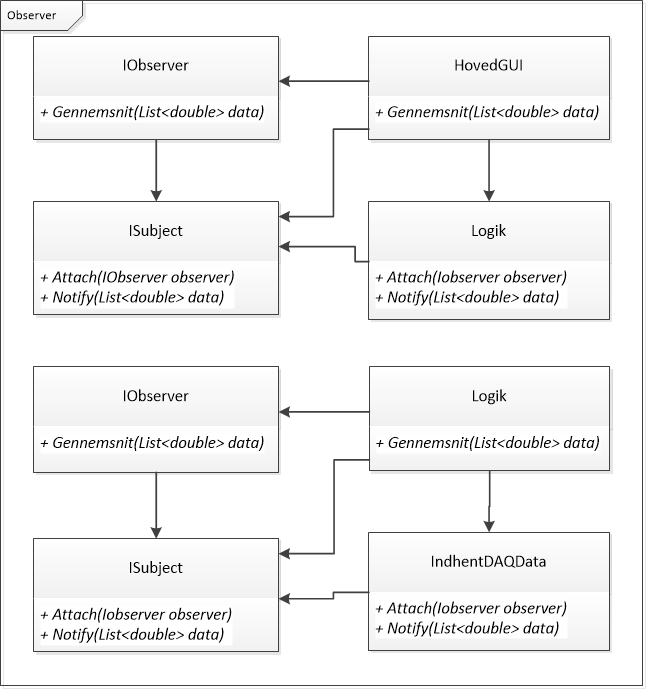
\includegraphics[width=0.8\textwidth]{Figurer/ObserverStrategy}
	\caption{Observer mønstre}
	%\label{fig:Skitse af implementeret observer mønster}
\end{figure}
Strategy mønstret indkapsler algoritmer og gør dem udskiftelige med hinanden. Det vil sige at en metode oprettes i et interface. Klasser vil så arve fra dette interface, afhængig af hvem der bruger metoden vil metoden så blive overskrevet i klassen og den nødvendige funktion tilføjet. I samarbejde med Observer-mønstret bruges det ved at Subject arver fra ISubject, og Observer arver fra IObserver. 
I projektet blev mønstrene i første omgang først benyttet fra logik-laget til præsentations-laget i forbindelse med at sende data til visning i graf. Men undervejs viste det sig nødvendigt også at implementere mønstrene fra data-laget til logik-laget, således at det kan kontrolleres hvor stor en mængde data der sendes op ad gangen. 

\subsubsection{Samplefrekvens}
Samplefrekvensen er som krav givet til 1000 Hertz. Hvilket svarer til at systemet modtager 1000 samples i sekunder. Varigheden af en sample er givet ved: 
\begin{ceqn}
\begin{equation}
\frac{1}{f_s}=\frac{1}{1000}=0.001 sek
\end{equation}
\end{ceqn}
Det har vist sig under arbejdet med softwaren, at systemet ikke kan følge med til at modtage så mange målinger i sekundet. Derfor er det valgt at skære i antallet af målinger pr. sekund der skal videre bearbejdes i logik-laget og udskrives i præsentations-laget. Antallet skæres ned til 50 målinger pr. sekund. Dette gøres ved at gennemsnittet af 20 målinger efter hinanden bestemmes, hvorefter gennemsnitsværdien returneres og gemmes i listen der sendes videre i systemet. Herefter findes så gennemsnittet af de næste 20 målinger og således fortsættende.   

\subsubsection{Nulpunktsjustering}
Formålet med en nulpunktsjustering er at flytte signalets offset enten op eller end, så det atmosfæriske tryk altid er placeret ved 0 volt på outputsignalet. Dette gøres ved at åbne for den tilsluttede transducer til systemet, så det atmosfæriske tryk måles. Ud fra denne værdi kan justeringsfaktoren så bestemmes ved, hvor x er det målte atmosfæriske tryk i volt modtaget gennem DAQ’en:
\begin{ceqn}
\begin{equation}
faktor_{jus}=0-(x)
\end{equation}
\end{ceqn}
Af ligningen ses det at justeringsfaktoren både vil kunne blive positiv og negativ, afhængig af om offset værdien skal rykkes op eller ned for at blive placeret i nul. Optimalt set vil det atmosfæriske tryk være en konstant værdi ved den samme måling, men det opleves at der er en smule støj på signalet og derfor vil den målte værdi være en tilnærmelse af det atmosfæriske tryk. Systemet ønskes nulpunktsjusteret for at sikre at alle de målte blodtrykssignaler har samme udgangspunkt. Hvilket gør at målingerne kan sammenlignes. Systemet foretager automatisk nulpunktsjusteringen når systemet startes ved at retunerer den første værdi fra DAQ'en, når der trykkes på knappen FORETAGET. Denne værdi er justeringsfaktoren der lægges til samtlige samples i det indhentede blodtrykssignal.

\subsubsection{Kalibrering}
Ved kalibrering ønskes det at bestemme hardwarens visningsfejl. I dette projekt betyder det at kalibreringsfaktoren fra volt til millimeter kviksølv bestemmes. Denne bestemmes ved at tilkoble en væskesøjle til systemet. Væskesøjlen fyldes med vand til den vil give et kendt mængde tryk på systemet angivet i mmHg. Herefter kan output i volt fra hardwaren måles. kalibreringsfaktor er givet ved:
\begin{ceqn}
\begin{equation}
faktor=\dfrac{x [mmHg]}{y [Volt]}
\end{equation}
\end{ceqn}
x angiver trykket fra væskesøjlen, denne hardcodes til 50 mmHg. y angiver den målte spændingsoutput på hardwaren. Optimalt set er kalibreringsfaktoren givet ved:
\begin{ceqn}
\begin{equation}
\dfrac{250 [mmHg]}{5 [V]}=50
\end{equation}
\end{ceqn}
hvor 250 mmHg er det maksimale blodtryk systemet kan måle og 5 Volt er maks spændingen i volt. Grafisk vil det se ud som vist på figur 3.8 under hardware modultest. Af figur 3.8 kan det aflæses at den optimale outputspænding ved 50 mmHg er 1 Volt. Kalibreringsfaktoren skal ganges på samtlige sample-værdier der kommer fra DAQ’en og som ønskes udskrevet på graf i display. 
Kaliberingen implementeres i softwaren ved brug af konfiguration. Forskeren beregner omsætningsværdien udfra ligning 3.16. Resultatet af denne beregning indtaster forsker i konfigurations xml-filen under App.settings. XML-filen kan tilgås uden opstart af systemet, derfor bliver kalibreringen uafhængig af hvornår systemet kører og kalibreringen kan dermed foretages på et vilkårligt tidspunkt. Værdien der ændres i XML-filen er den tilhørende "Value" til "KalibreringsKoefficient". Den er markeret med grøn firkant omkring på figur 3.24.
\begin{figure}[H]
	\centering
	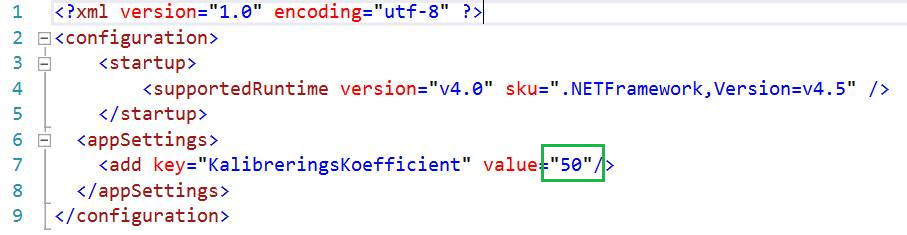
\includegraphics[width=1.0\textwidth]{Figurer/XMLConfig}
	\caption{Konfigurations XML-fil}
	%\label{fig:Konfigurations XML-fil til kalibrering}
\end{figure}
Metoden Kalibrering() i Kalibreringsklassen, som er en del af logik-laget læser så "Kalibreringskoefficienten" fra konfigurations-filen hver gang kalibreringsfaktoren skal ganges på et signal. 

Det er vigtigt at pointere at nulpunktsjusteringsfaktoren lægges til samtlige værdier i signalet førend at kalibreringsfaktoren ganges på. Dette udføres i kodens logik-lag.
 
\subsubsection{Digitalt Filter}
\cite{DSBsoft} Formålet med implementering af et digitalt filter er at fjerne støj fra det indhentede signal. Dette gøres ved at udglatte signalet. Til dette kan en række forskellige filtre benyttes. Vi har valgt at implementere et glidende middelværdifilter (moving average filter). Fordelen ved dette filter er at det er simpelt at forstå og at det er optimalt at bruge på signaler i tidsdomænet. Skulle signalet være vist i frekvensdomænet ville valget have faldet på et helt andet filter. 

Det glidende middelværdifilter fungerer ved midling af en række punkter fra inputsignalet for at frembringe hvert punkt i outputsignalet. Hvilke punkter der tages fra inputsignalet vil flytte sig en plads for hvert beregnet outputsignal punkt, heraf kommer den glidende effekt. Matematisk er filtret givet ved:
\begin{ceqn}
\begin{equation}
y[i]=\frac{1}{M}\cdot\sum\limits_{j=0}^{M-1} x[i+j]
\end{equation}
\end{ceqn}

Hvor x[] er inputsignalet, y[] er outputsignalet og M er antallet af punkter der benyttes i det glidende middelværdifilter. Denne beregning benytter sig udelukkende af punkter placeres på den samme side af output sample nummeret, hvilket vil føre til en relativ forskydning mellem input og output. M sættes til 5. Implementeringen af filtret er vist i et aktivitetsdiagram på figur 3.25.

\begin{figure}[H]
	\centering
	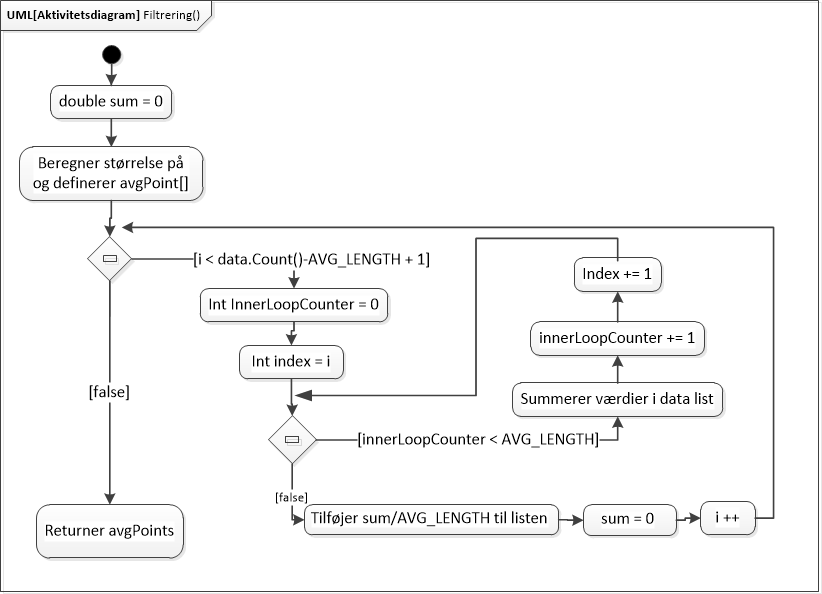
\includegraphics[width=1.0\textwidth]{Figurer/AktFiltrering}
	\caption{Aktivitetsdiagram af metoden Filtrering()}
	%\label{fig:Aktivitetsdiagram for metoden filtrering() i klassen Digitalt filter}
\end{figure}

Måden hvorpå filtret er implementeret gør at der ikke sker en filtrering af de første fire samples, det ses af følgende i koden. AVG\_LENGTH er defineret til 5, og mængden af punkter der benyttes i filtret i ligning 3.18 svarer dette til M.

\begin{figure}[H]
	\centering
	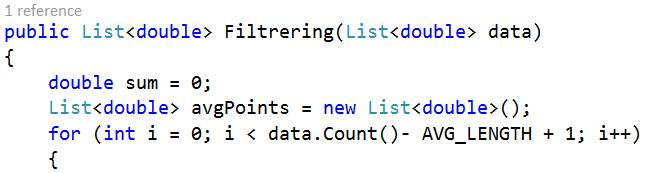
\includegraphics[width=0.7\textwidth]{Figurer/UdsnitFilter}
	\caption{Udsnit af koden til det glidende middelværdifilter}
	%\label{fig:Kode udsnit af det glidende middelværdifilter}
\end{figure}

Det ses at der skal være minimum 5 samples i data.Count førend at listen avgPoints oprettes. Det er en begrænsning vi er opmærksom på, men som accepteres da de første fire samples ved visning i graf er kørt så hurtigt igennem, at det ikke skaber en begrænsning for brugen af systemet for forsker. Optimalt set vil der sættes en begrænsning på filtret således når første måling modtages vil gennemsnittet findes af en sample, dernæst af to samples, tre samples osv. Indtil der er fem samples og gennemsnittet vil så altid bestemmes af de fem seneste samples. 

Systemet gør det muligt for forsker selv at vælge om signalet ønskes vist filtreret eller ufiltreret. Dette vælges på brugergrænsefladen. Vælges visning af det ufiltrede signal sendes det indhentede signal naturligvis ikke gennem det digitale filter. Det er muligt at skifte mellem filtreret og ufiltreret signal, mens systemet kører. I det tilfælde skifter hele det viste signal til det valgte, da alt data i listen der indhentes dermed skifter. Filtreringen vil dermed ikke vise sig som en løbende kurve grafisk.

\subsubsection{Analyse}
Analyse dækker over indhentningen af de systoliske-, diastoliske- og puls-værdi ud fra blodtrykssignalet. Dette er implementeret i en klasse kaldet Analyse. Heri er placeret metoder for henholdsvis systole og diastole. I en blodtrykskurve er den systoliske værdi givet ved maximum på kurven og den diastoliske er givet ved minimums værdien på kurven. \\
Metoderne bestemmer derfor den maksimale værdi og den mindste værdi i listen, der medtages som parametre til metoderne. Listen der bruges som parametre er UILIST indeholdende 350 tal ad gangen. UILIST er listen der sendes fra logik-laget til præsentations-laget med de behandlede data, som vises i grafen. I præsentations-laget er implementeret en timer, der håndterer at de systoliske- og diastoliske værdier i display kun opdateres hvert 3 sekund. I løbet af 3 sekunder vil der være gennemløbet 3-5 blodtryksperioder, afhængig af pulsfrekvensen. Dermed vil samtlige systoliske og diastoliske værdier ikke blive udskrevet. Intervallet på 3 sekunder er valgt da det er passende tid til at kunne nå og aflæse den pågældende værdi.

I forhold til implementering af puls er der gjort en række overvejelser og mulige løsninger. Puls er defineret ved slag pr. minut og på en puls vil der være en systole og diastole. Pulsen må derfor kunne bestemmes ved at tælle antallet af systoliske værdier på 6 sekunder, antallet ganges så med 10 for at få den rette enhed. Udfordringer er dog opstået i forhold til at kunne bestemme præcist hvornår der er gået 6 sekunder i programmet. En anden mulighed er også at bestemme pulsen ved at finde antallet af samples mellem to systoliske værdier. Omregnes samples så til sekunder og ganges op til et minut, må dette være ligmed måleobjektets øjeblikkelige puls. Det er dog ikke lykkedes at omsætte overvejelserne til kode, og pulsen er dermed ikke blevet implementeret ved projekt aflevering.

\subsubsection{Beregnings metode}
Metoden updateListe() er den vigtigste metode i logik-laget. Den er placeret i logikklassen. Metoden har til ansvar at tage højde for nulpunktsjustering og kalibering ved beregning. Derudover har den til ansvar at lægge data i en liste med 300 pladser, der kan vises i graf på display. Til sidst tjekker metoden om radiobuttom for filtreret eller ufiltreret signal er checked og sender listen gennem filtret, hvis filtret signal er valgt inden listen med Notify() sendes til præsentationslaget. Metodens aktivitetsdiagram er givet ved:
\begin{figure}[H]
	\centering
	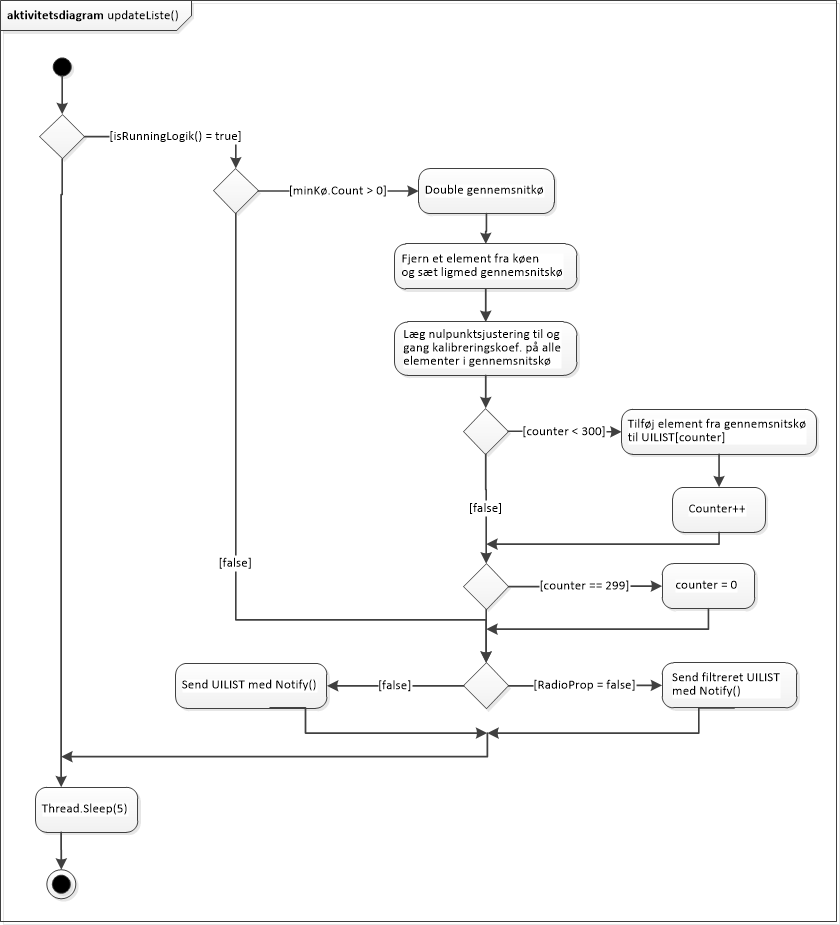
\includegraphics[width=1.0\textwidth]{Figurer/AktUpdateListe}
	\caption{Aktivitetsdiagram for metoden updateListe()}
	%\label{fig:Aktivitetsdiagram for metoden updateListe()}
\end{figure}

\subsubsection{Database}
I systemet er der implementeret en lokal database. Databasen er oprettet gennem host webhotel10.iha.dk. Formålet med databasen er at lagre det målte blodtrykssignals rådata. Det er valgt at implementere databasen som typen SQL, da denne database-type indeholder de funktioner som er nødvendige for dette system. Data gemmes i denne type database i tabeller. Indledningsvis for at oprette den nødvendige tabel defineres en type til hver værdi. SQL-koden til oprettelse af tabel er vist på figur xx.
\begin{figure}[H]
	\centering
	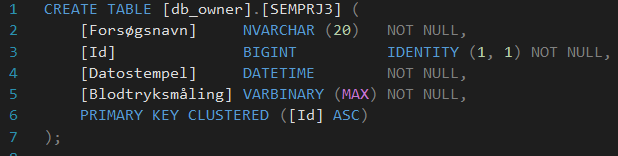
\includegraphics[width=0.7\textwidth]{Figurer/SQLDatabase}
	\caption{SQL-kode til oprettelse af tabeller i database}
	%\label{fig:SQL-kode til oprettelse af tabeller i lokal database}
\end{figure}
Forsøgsnavnen referer til det forsøgsnavn der indtastes i GUI ved påbegyndelse af en ny måling. Dette er af typen NVARCHAR(20), hvilket betyder at forsøgsnavnet maksimalt kan være 20 tegn langt. Id er defineret som primær nøgle, det betyder at denne er unik for hver enkelt sekvens i database, og Id der vil referes til mellem tabeller i databasen, hvis flere tabeller var nødvendigt. \\  
Et blodtrykssignal indeholder en stor mængde datapunkter, derfor gemmes signalet i en VARBINARY, hvor en række binære datapunkter gemmes som en enkelt enhed i databasen. Dette er valgt for at spare på data pladsen i databasen. Denne type besværliggør dog, at få vist hvilke værdier blodtrykssignalets datapunkter består af. \\
Databasen er implementeret således at flere sekvens af den samme måling kan gemmes uden at systemet skal startes forfra. Dette er smart for forsker, hvis der testet flere ting på det samme signal.  

\subsection{Modultest}
